\documentclass[tikz,border=10pt]{standalone}
\begin{document}
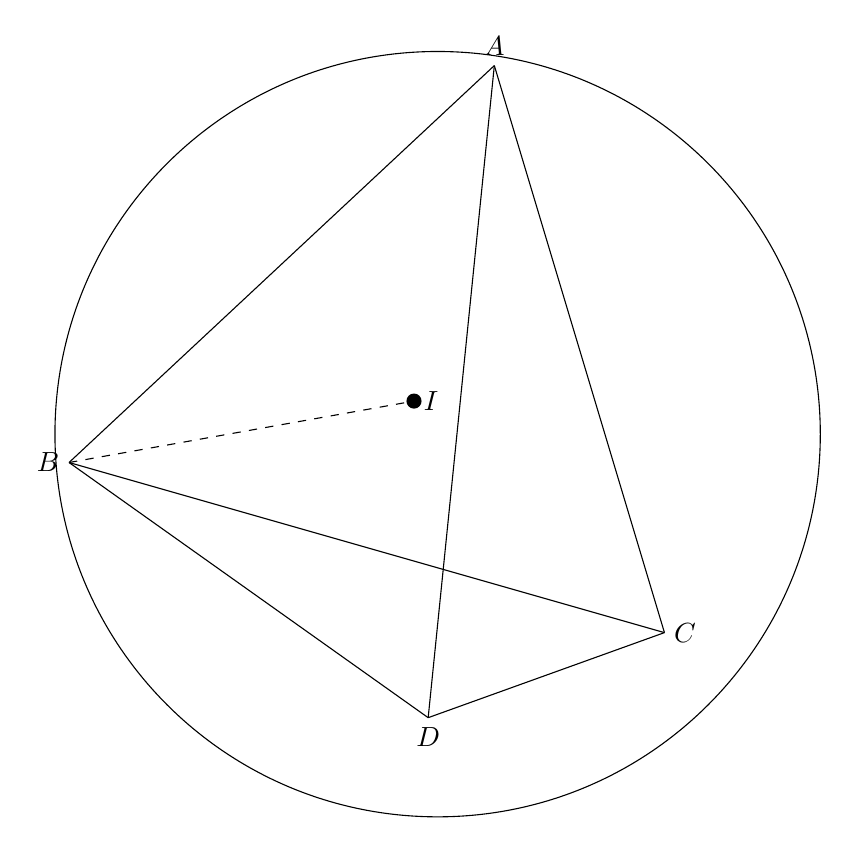
\begin{tikzpicture}[scale=1.2]

\coordinate (O) at (0,0);
\coordinate (A) at (0.6,3.9);
\coordinate (B) at (-3.9,-0.3);
\coordinate (C) at (2.4,-2.1);
\coordinate (D) at (-0.1,-3.0);
\coordinate (I) at (-0.25,0.35);

\draw (O) circle[radius=4.05];

\draw (A) -- (B);
\draw (A) -- (C);
\draw (A) -- (D);
\draw (B) -- (C);
\draw (B) -- (D);
\draw (D) -- (C);
\draw[dashed] (B) -- (I);

\fill (I) circle[radius=0.08];

\node[above] at (A) {$A$};
\node[left] at (B) {$B$};
\node[right] at (C) {$C$};
\node[below] at (D) {$D$};
\node[right] at (I) {$I$};

\end{tikzpicture}
\end{document}
